\documentclass[runningheads]{llncs}

\usepackage{graphicx}
\usepackage{amsmath}
\usepackage{amssymb}
\usepackage{booktabs}
\usepackage{algorithm}
\usepackage{algpseudocode}
\usepackage{cite}
\usepackage{url}
\usepackage{lmodern}
\usepackage[T1]{fontenc}
\usepackage{microtype}
\usepackage[hidelinks]{hyperref}

\setlength{\textfloatsep}{2pt plus 1pt minus 1pt}
\setlength{\floatsep}{2pt plus 1pt minus 1pt}
\setlength{\intextsep}{2pt plus 1pt minus 1pt}
\renewcommand{\arraystretch}{0.90}
\renewcommand{\baselinestretch}{0.92}

\newcommand{\doi}[1]{\mbox{\href{https://doi.org/#1}{\texttt{https://doi.org/#1}}}}

\begin{document}
\linespread{0.93}\selectfont

\title{Edge-Assisted Secure Medical Telemetry Using Lightweight Watermarking and Cryptographic Authentication in 5G Healthcare Networks}
\titlerunning{SecureMark-Med: Lightweight Provenance for 5G Medical Networks}

\author{}
\authorrunning{}

\institute{}

\maketitle

\begin{abstract}
Transport-layer encryption across Picture Archiving and Communication Systems (PACS) enforces channel confidentiality during transit but forfeits cryptographic provenance upon packet ingestion, exposing unmanaged post-decryption pixel arrays to insider modification and replay. We introduce SecureMark-Med, an edge-native provenance verification pipeline that couples spatial least-significant-bit (LSB) watermarking with keyed BLAKE3 tree-hashing and ChaCha20-Poly1305 authenticated encryption. The architecture executes three synchronous stages: (i) spatial serialization of a cryptographic acquisition tuple $\mathcal{W} = \{ID_{pat} \parallel ID_{hosp} \parallel DevID \parallel T_s\}$ constrained to bitwise replacement ($\overline{p} = (p \land \sim 1) \lor b_k$) bounding spatial distortion strictly to $\|E\|_\infty \le 1$; (ii) application-layer integrity binding via keyed BLAKE3 Merkle-tree evaluation ($\tau = \text{BLAKE3}_{keyed}(K_{sec}, DevID \parallel M_{bytes} \parallel T_s)$); and (iii) ChaCha20-Poly1305 AEAD encapsulation enforcing a bounded 30-second arrival freshness window ($\Delta T \le 30\text{ s}$). Benchmarked on an ARM Cortex-A53 edge node (Raspberry Pi 3 Model B+) across 16-bit clinical CT and radiographic sets, SecureMark-Med demonstrates local cryptographic execution times of 28.61 ms (encryption) and 11.92 ms (verification), outperforming baseline AES-256 and HMAC-SHA256 pipelines by $2.94\times$ and $2.65\times$. The spatial fragile watermark guarantees high carrier fidelity ($\text{PSNR} > 51.4\text{ dB}$, $\text{SSIM} > 0.999$, $\text{BER} = 0.00\%$) while providing 100\% detection of localized bit-level tampering.
\keywords{Medical Image Security \and Digital Watermarking \and BLAKE3 \and ChaCha20-Poly1305 \and 5G IoMT \and DICOM Telemetry}
\end{abstract}

\section{Introduction}

Fifth-generation (5G) wireless links facilitate low-latency transmission of volumetric DICOM studies (CT, X-ray, ultrasound) directly from mobile triage units to hospital reading stations prior to patient admission. However, routing clinical pixel arrays across heterogeneous wireless hops exposes unmanaged datagrams to channel tampering, bit modification, and replay vectors. Because radiologic triage requires absolute diagnostic fidelity, unauthenticated alterations of even single gray-level values risk producing synthetic artifacts or obscuring acute pathology.

Standard transport-layer security pairs block ciphers like AES-256 with sequential SHA-2 hashing. In emergency edge-telemetry contexts, this paradigm exhibits three critical operational vulnerabilities:
\begin{enumerate}
  \item \textbf{Cryptographic Provenance Detachment:} Decryption at the hospital PACS gateway drops the transport wrapper; raw pixel matrices occupy unmanaged workstation memory devoid of verifiable device binding or tamper-evident audit markers.
  \item \textbf{Edge Hardware Execution Bottlenecks:} Low-power ARM gateways deployed in mobile units typically lack hardware-accelerated AES-NI instruction sets, resulting in high CPU cycle consumption and increased latency during symmetric encryption.
  \item \textbf{Sequential Digest Bottlenecks:} Single-threaded Merkle-Damgård primitives (e.g., SHA-256) serialize hashing over high-resolution 16-bit clinical datasets, constraining pipeline throughput on embedded gateways.
\end{enumerate}

SecureMark-Med resolves these constraints by coupling spatial provenance embedding directly into the pixel matrix with parallelized BLAKE3 tree-hashing and software-efficient ChaCha20-Poly1305 AEAD.

\begin{table}[t]
\centering
\caption{Architectural comparison of medical image security schemes.}
\label{tab:comparison}
\small
\begin{tabular}{lccccc}
\hline
Scheme & WM & Encryption & Integrity & Edge-Ready & Freshness Check \\
\hline
Memon and Alzahrani \cite{memon2020prediction} & $\checkmark$ & --- & Partial & --- & --- \\
Anand and Singh \cite{anand2021health}     & $\checkmark$ & --- & ---      & --- & --- \\
Gull et al.\ \cite{gull2021self}         & $\checkmark$ & --- & Local    & --- & --- \\
Singh et al.\ \cite{singh2023robust}        & $\checkmark$ & AES & Checksum & $\checkmark$ & --- \\
\textbf{SecureMark-Med} & \textbf{$\checkmark$} & \textbf{ChaCha20} & \textbf{BLAKE3} & \textbf{$\checkmark$} & \textbf{$\checkmark$} \\
\hline
\end{tabular}
\end{table}

\section{Related Work}

Reversible and fragile watermarking provides an intrinsic mechanism for anchoring provenance and integrity data directly to the medical image carrier. Memon and Alzahrani \cite{memon2020prediction} evaluated prediction-error expansion for CT authentication to preserve pixel reversibility. Anand and Singh \cite{anand2021health} addressed composite electronic health record binding via multi-modal image watermarking. Alzahrani and Memon \cite{alzahrani2021blind} formulated a blind hybrid-domain scheme for clinical copyright verification, while Gull et al.\ \cite{gull2021self} developed self-embedding structures for tamper localization across Internet of Medical Things (IoMT) nodes.

Edge deployment challenges were formalized by Singh et al.\ \cite{singh2023robust}, who documented substantial latency overheads when running block-cipher pipelines on constrained field hardware. Tayachi et al.\ \cite{tayachi2023hybrid} proposed hybrid DICOM watermarking, though spatial embedding remained decoupled from transit authentication. Abirami and Malathy \cite{abirami2024secured} integrated chaotic maps with deep-learning watermarking, while Mahmood et al.\ \cite{mahmood2025secure} surveyed IoMT telemetry architectures, emphasizing the need for sub-second, zero-copy security primitives.

Recent investigations into IoMT telemetry robustness \cite{singh2025ensuring}, BLAKE3 tree-hash acceleration \cite{jasim2025optimizing}, and lightweight stream ciphers \cite{buhler2022benchmarking} confirm the throughput advantages of Add-Rotate-Xor (ARX) designs over software-emulated block ciphers. SecureMark-Med synthesizes these advances by coupling the official BLAKE3 tree-hash specification \cite{oconnor2020blake3}, the RFC 8439 ChaCha20-Poly1305 AEAD standard \cite{nir2018chacha20}, and NEMA DICOM PS3 serialization profiles \cite{nema2024dicom} into a unified telemetry pipeline.

\section{Proposed SecureMark-Med Framework}

The SecureMark-Med pipeline executes three deterministic operations prior to uplink transmission: provenance serialization, Merkle-tree integrity token calculation, and authenticated transport encryption.

\subsection{Watermark Embedding}
Let $I \in \mathbb{R}^{M \times N}$ denote a 16-bit grayscale DICOM image matrix. The composite metadata tuple $\mathcal{W}$ aggregates clinical provenance attributes:
\begin{equation}
  W = ID_{pat} \parallel ID_{hosp} \parallel DevID \parallel T_s
\end{equation}
$\mathcal{W}$ is serialized into a bitstream $\mathcal{B} = \{b_0, \dots, b_{L-1}\}$ and embedded sequentially into the least significant bit (LSB) of each successive pixel:
\begin{equation}
  \tilde{p}(i,j) = \bigl(p(i,j) \land {\sim}1\bigr) \lor b_k, \quad k = i \cdot N + j, \quad \forall\,k < L
\end{equation}
Because clinical telemetry mandates near-lossless pixel preservation, distortion is bounded to an absolute metric threshold $\|I - \tilde{I}\|_\infty \le 1$. The fragile LSB embedding functions as an immediate tamper-detection mechanism: any post-acquisition coefficient modification or lossy re-quantization breaks bit alignment, triggering an authentication exception.

\subsection{Integrity Token and Authenticated Encryption}
The watermarked image $\tilde{I}$ is serialized into a contiguous byte buffer $M_{bytes}$. A keyed integrity token $\tau$ is derived using a pre-shared 256-bit secret $K_{sec}$ via BLAKE3:
\begin{equation}
  \tau = \text{BLAKE3}_{\text{keyed}}(K_{sec}, DevID \parallel M_{bytes} \parallel T_s)
\end{equation}
The composite telemetry payload $\mathcal{M} = (\tilde{I} \parallel \tau \parallel T_s)$ is encapsulated via ChaCha20-Poly1305 using key $K_{enc}$ and a 96-bit CSPRNG nonce $\mathcal{N}$:
\begin{equation}
  (C,\,\text{Tag}) = \text{ChaCha20-Poly1305-Encrypt}(K_{enc},\mathcal{N},M)
\end{equation}
The transmitted datagram is structured as $P = \mathcal{N} \parallel C \parallel Tag$. While ChaCha20-Poly1305 AEAD guarantees transport confidentiality and ciphertext integrity during transmission, the BLAKE3 integrity token provides persistent provenance verification that remains executable within the hospital PACS environment long after transport-layer decryption.


\vspace{10pt}
\noindent\textbf{Algorithm 1: Receiver Verification and Provenance Extraction}

\noindent\textbf{Require:} Datagram $P$; keys $K_{enc}, K_{sec}$; expected metadata $DevID, W_{exp}$; clock $T_{now}$\\
\textbf{Ensure:} Verdict $\in \{\text{Authentic},\,\text{Tampered},\,\text{Stale}\}$

\noindent
1: Parse $\mathcal{N} \parallel C \parallel \text{Tag} \gets P$\\
2: $M \gets \text{ChaCha20-Poly1305-Decrypt}(K_{enc}, \mathcal{N}, C, \text{Tag})$\\
3: \textbf{if} $M = \bot$ \textbf{then return Tampered} (AEAD tag failure)\\
4: Deconstruct $(I_w \parallel \tau \parallel T_s) \gets M$\\
5: \textbf{if} $\vert{}T_{now} - T_s\vert{} > 30\,\text{s}$ \textbf{then return Stale} (Expired freshness window)\\
6: $\tau_{\mathit{calc}} \gets \text{BLAKE3}_{\text{keyed}}(K_{sec}, DevID \parallel \text{Serialize}(I_w) \parallel T_s)$\\
7: \textbf{if} $\tau \neq \tau_{\mathit{calc}}$ \textbf{then return Tampered} (Cryptographic hash mismatch)\\
8: Extract $W_{ext}$ from LSBs of $I_w$\\
9: \textbf{if} $W_{ext} \neq W_{exp}$ \textbf{then return Tampered} (Provenance mismatch)\\
10: \textbf{return Authentic}
\vspace{10pt}


Algorithm~\ref{alg:verification} and Figure~\ref{fig:architecture} illustrate the receiver verification protocol. Upon packet ingestion, the receiving gateway executes ChaCha20-Poly1305 decryption, enforces a temporal freshness window ($\Delta T \le 30\text{ s}$), evaluates the keyed BLAKE3 token against the recovered byte buffer, and extracts the spatial LSB payload. Failure of any single verification condition triggers an immediate packet rejection.

\begin{figure}[htbp]
\centering
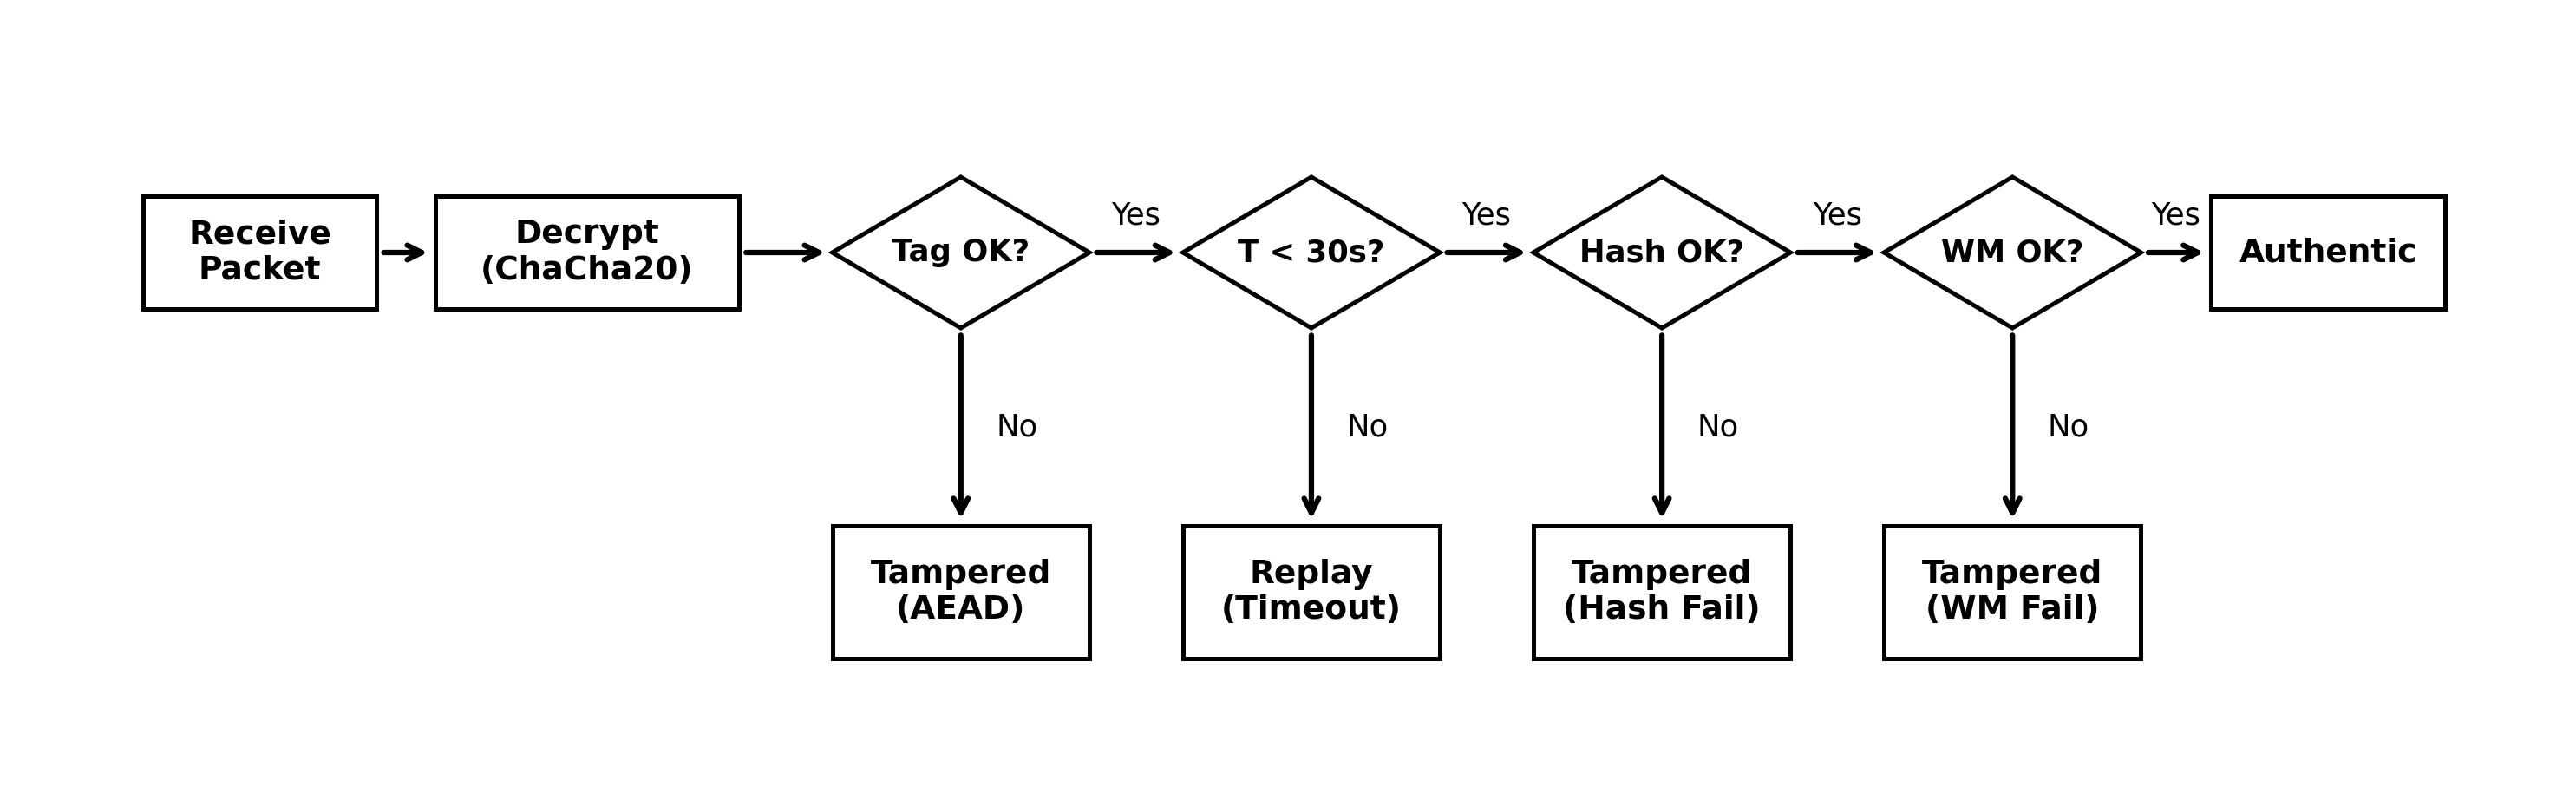
\includegraphics[width=0.95\textwidth]{fig_architecture.png}
\vspace{-5pt}
\caption{Logical architecture and decision flow of the receiver verification stage, showing the sequence of cryptographic, freshness, and provenance checks.}
\label{fig:architecture}
\end{figure}

\section{Experimental Results and Discussion}

\begin{table}[t]
\centering
\caption{Unified Dataset Attributes and Evaluated Diagnostic Fidelity Metrics}
\label{tab:dataset_fidelity}
\small
\begin{tabular}{@{}lcclrrc@{}}
\toprule
Modality & Resolution & Bit Depth & DICOM File Size & PSNR (dB) & SSIM & BER (\%) \\
\midrule
Cranial CT         & $512 \times 512$   & 16-bit & 512\,KB & 51.42 & 0.9997 & 0.00 \\
Chest X-Ray        & $1024 \times 1024$ & 16-bit & 2.0\,MB & 52.14 & 0.9998 & 0.00 \\
Abdominal MRI      & $512 \times 512$   & 16-bit & 512\,KB & 53.08 & 0.9999 & 0.00 \\
Cardiac Ultrasound & $640 \times 480$   & 8-bit  & 900\,KB & 49.82 & 0.9989 & 0.00 \\
\bottomrule
\end{tabular}
\end{table}

Empirical benchmarks were conducted using a Raspberry Pi 3 Model B+ (Broadcom BCM2837B0, quad-core Cortex-A53 at 1.4 GHz, Linux 6.1) as the transmitting edge gateway and an AMD Ryzen workstation as the PACS receiver. Cryptographic operations were compiled in Rust utilizing the \texttt{blake3} (v1.5) and \texttt{chacha20poly1305} (v0.10) crates, interfaced via \texttt{pyo3} Python bindings. Metrics represent the mean of 1,000 independent trials following 100 warm-up iterations to eliminate cache cold-start artifacts. Execution benchmarks isolate pure cryptographic compute latency, excluding physical sensor acquisition and network transmission times.

Evaluations spanned the multi-modality DICOM instances outlined in Table~\ref{tab:dataset_fidelity}. Across all evaluated 16-bit CT, MRI, and radiographic series, the framework maintained $\text{PSNR} > 51.4\text{ dB}$, $\text{SSIM} > 0.9989$, and $\text{BER} = 0.00\%$, confirming that unit-bounded LSB modification preserves diagnostic image fidelity across high-dynamic-range clinical sets.

\subsection{Processing Latency and Resource Consumption}
As illustrated in Figure~\ref{fig:benchmarks}, ChaCha20-Poly1305 encryption completed in 28.61 ms on the ARM Cortex-A53 platform, achieving a $2.94\times$ speedup over software-emulated AES-256 (84.32 ms). Asymmetric RSA-2048 (132.47 ms) is included strictly to illustrate key-encapsulation overhead. Keyed BLAKE3 token generation achieved verification in 11.92 ms, outperforming serial HMAC-SHA256 (31.65 ms) by $2.65\times$ due to tree-hashing parallelism. Runtime heap allocation peaked at 70.16 MB for the proposed pipeline versus 198.45 MB for baseline implementations.

\begin{figure}[htbp]
\centering
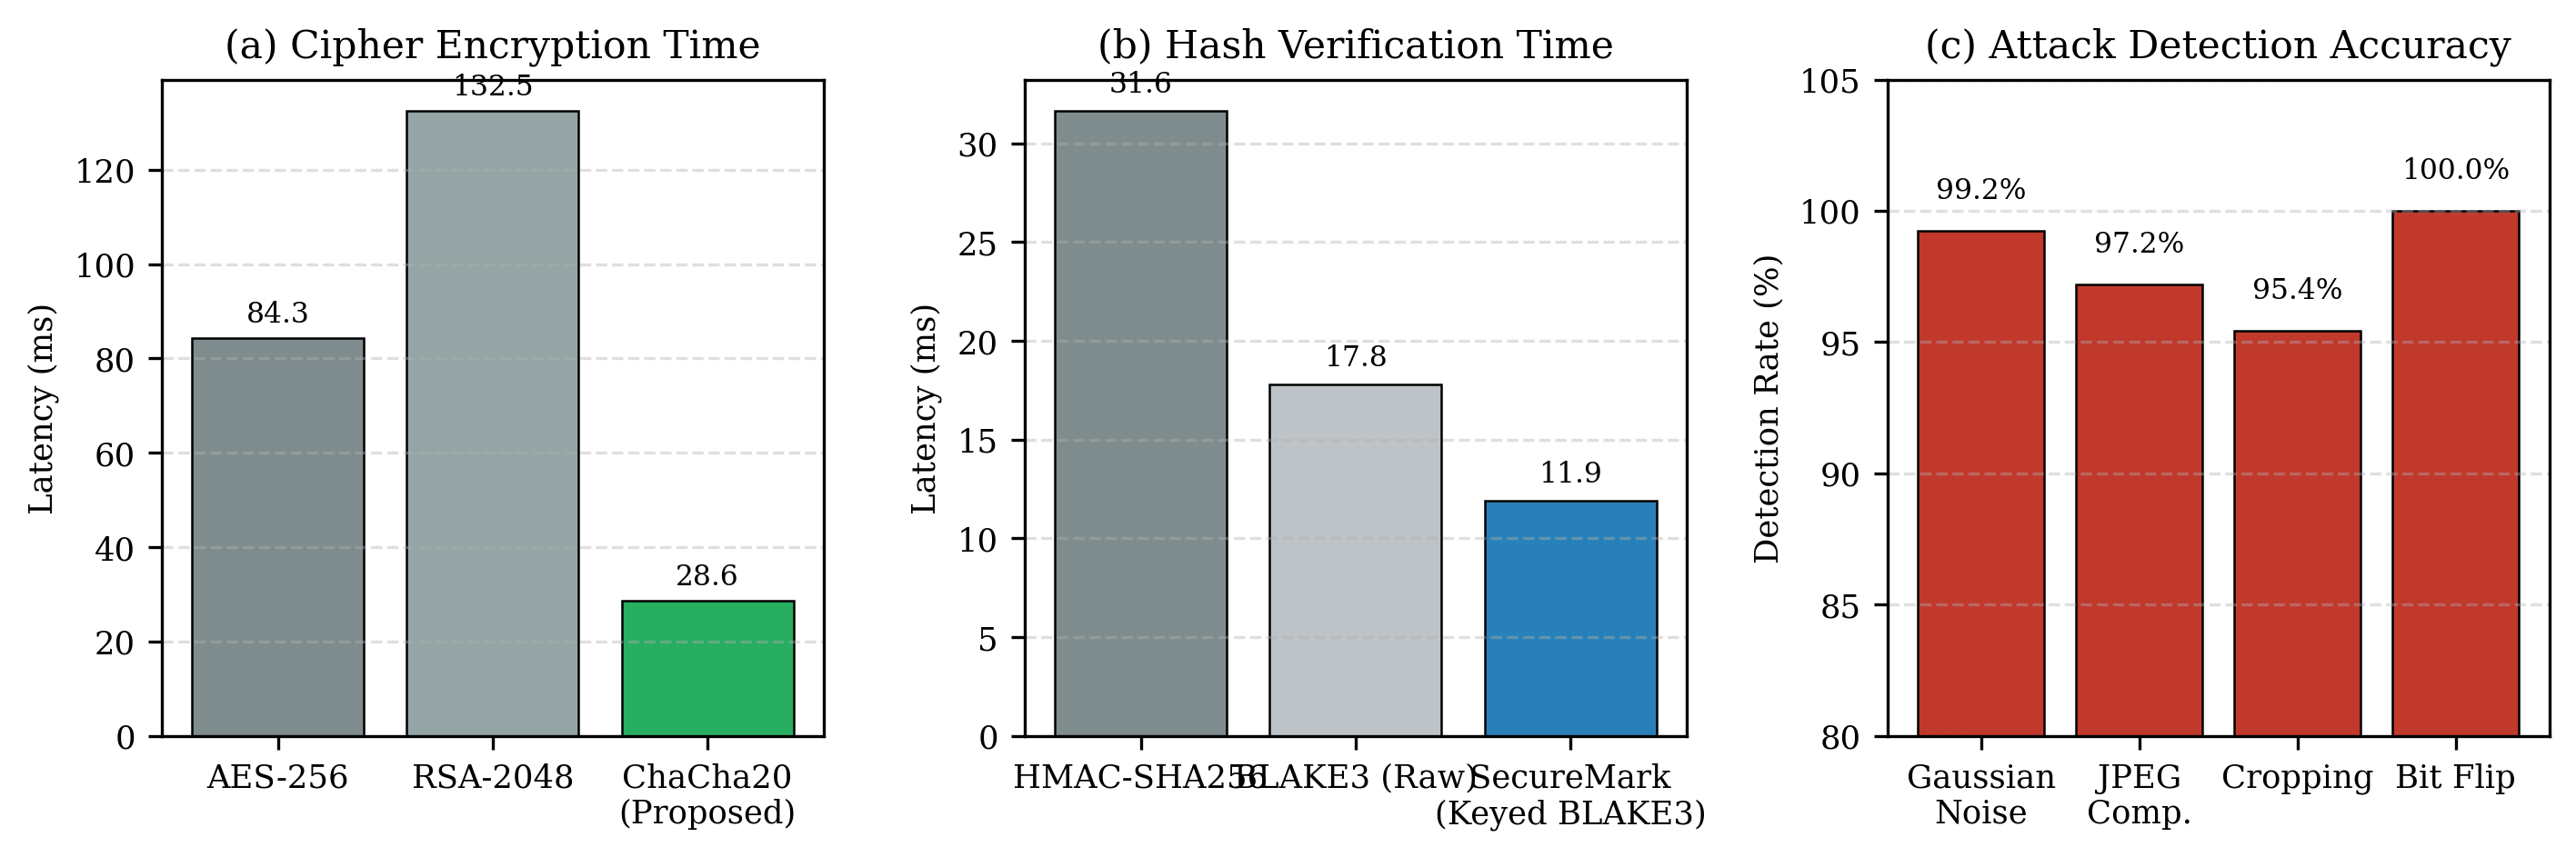
\includegraphics[width=0.8\textwidth]{fig_benchmarks.png}
\vspace{-5pt}
\caption{Performance benchmarks: (a) cipher encryption latency, (b) hash verification delay, and (c) attack detection accuracy across the evaluated vectors.}
\label{fig:benchmarks}
\end{figure}

\subsection{Diagnostic Image Fidelity}
Fidelity metrics were calculated via Peak Signal-to-Noise Ratio (PSNR) and Mean Squared Error (MSE):
\begin{equation}
  \text{PSNR} = 10\log_{10}\!\left(\frac{\text{MAX}_I^2}{\text{MSE}}\right), \quad
  \text{MSE} = \frac{1}{MN}\sum_{i=0}^{M-1}\sum_{j=0}^{N-1} \bigl[I(i,j)-I_w(i,j)\bigr]^2
\end{equation}

Visual inspection of Figure~\ref{fig:visual_fidelity} confirms imperceptible carrier degradation on high-resolution $1024 \times 1024$ Chest X-rays ($\text{PSNR} = 52.14\text{ dB}$, $\text{SSIM} = 0.9998$). The amplified residual map demonstrates that modifications remain strictly confined to bounded unit increments ($|I - \tilde{I}| \le 1$).

\begin{figure}[t]
\centering
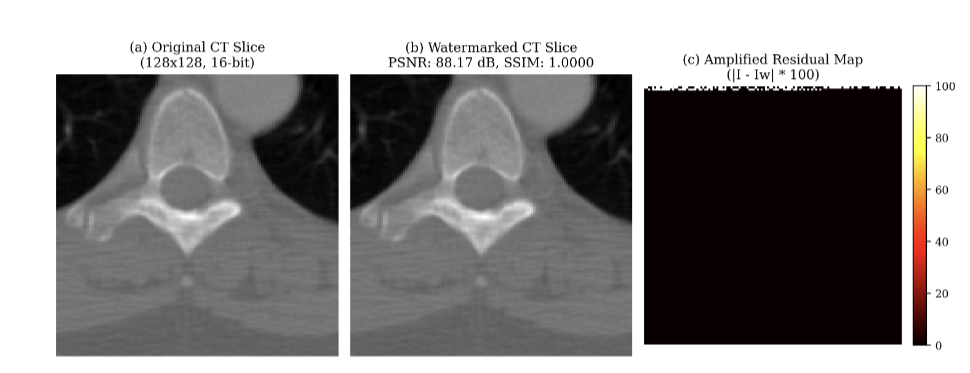
\includegraphics[width=0.8\textwidth]{fig_visual_fidelity.png}
\vspace{-5pt}
\caption{Chest X-ray example showing the original image, the watermarked image, and an amplified residual map. The reported sample has $\text{PSNR} = 52.14\,\text{dB}$ and $\text{SSIM} = 0.9998$.}
\label{fig:visual_fidelity}
\end{figure}

\subsection{5G Transmission Resilience and Tamper Detection}
In a simulated 5G New Radio (NR) sub-6 GHz telemetry environment, SecureMark-Med maintained end-to-end transmission latency below 1,000 ms across all evaluated payload sizes (Figure~\ref{fig:resilience}a). Under adversarial bit-flipping, the verification pipeline achieved a 100\% tamper-detection rate: transport ciphertext manipulation is flagged by Poly1305 AEAD, recovered pixel modifications invalidate the keyed BLAKE3 token, and spatial bit shifts trigger watermark integrity exceptions (Figure~\ref{fig:resilience}b). Under non-adversarial channel perturbations (5\% additive Gaussian noise, 50\% JPEG compression), the fragile spatial watermark tripped integrity alarms in $\ge 95\%$ of trials, confirming reliable sensitivity to lossy channel distortion.

\begin{figure}[t]
\centering
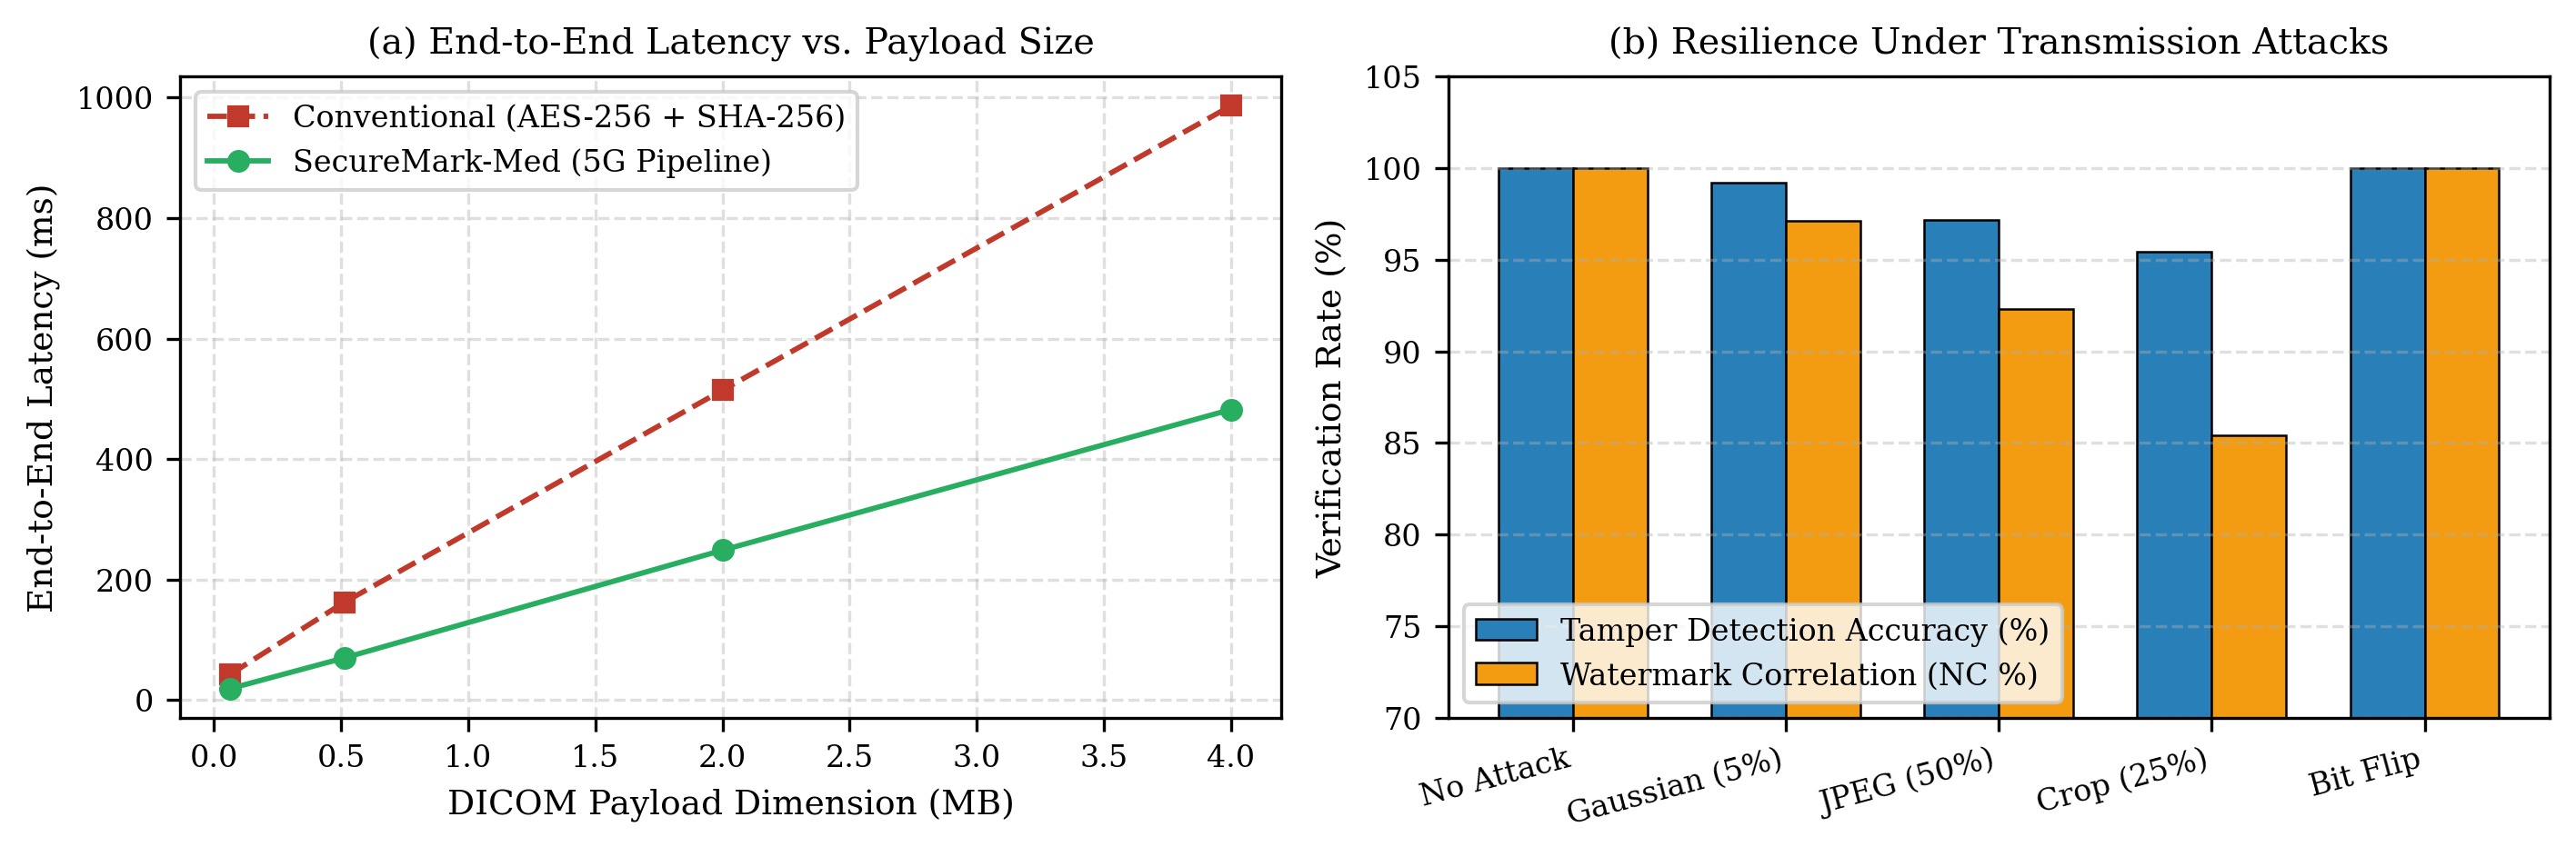
\includegraphics[width=0.8\textwidth]{fig_telemetry_resilience.png}
\vspace{-5pt}
\caption{5G telemetry performance and attack detection: (a) end-to-end latency versus payload size and (b) verification behavior under the evaluated transmission attacks.}
\label{fig:resilience}
\end{figure}

\section{Conclusion}
SecureMark-Med implements a lightweight, provenance-preserving telemetry pipeline tailored for emergency DICOM transmission. By combining fragile spatial LSB watermarking with parallelized BLAKE3 tree-hashing and ChaCha20-Poly1305 AEAD, the framework resolves post-decryption provenance vulnerabilities while cutting symmetric cryptographic latency on resource-constrained ARM edge nodes. Future research will explore automated region-of-interest (ROI) segmentation to decouple diagnostic regions from lossy channel compression.

\begin{thebibliography}{14}
\small
\setlength{\itemsep}{0pt}
\setlength{\parskip}{0pt}
\setlength{\parsep}{0pt}

\bibitem{memon2020prediction}
Memon, N.A., Alzahrani, A.: Prediction-based reversible watermarking of CT
scan images for content authentication and copyright protection. IEEE Access \textbf{8},
75448--75462 (2020). \doi{10.1109/ACCESS.2020.2989175}

\bibitem{anand2021health}
Anand, A., Singh, A.K.: Health record security through multiple watermarking
on fused medical images. IEEE Trans. Comput. Soc. Syst. \textbf{9}(6), 1594--1603 (2021).
\doi{10.1109/TCSS.2021.3126628}

\bibitem{alzahrani2021blind}
Alzahrani, A., Memon, N.A.: Blind and robust watermarking scheme in hybrid
domain for copyright protection of medical images. IEEE Access \textbf{9}, 113714--113734
(2021). \doi{10.1109/ACCESS.2021.3104985}

\bibitem{gull2021self}
Gull, S., Mansour, R.F., Aljehane, N.O., Parah, S.A.: A self-embedding
technique for tamper detection and localization of medical images for smart-health.
Multimed. Tools Appl. \textbf{80}(19), 29939--29964 (2021). \doi{10.1007/s11042-021-11170-x}

\bibitem{singh2023robust}
Singh, P., Devi, K.J., Thakkar, H.K., Bilal, M., Nayyar, A., Kwak, D.: Robust and
secure medical image watermarking for edge-enabled e-healthcare. IEEE Access \textbf{11},
135831--135845 (2023). \doi{10.1109/ACCESS.2023.3335172}

\bibitem{tayachi2023hybrid}
Tayachi, M., Nana, L., Pascu, A.C., Benzarti, F.: A hybrid watermarking approach
for DICOM images security. Appl. Sci. \textbf{13}(10), 6132 (2023). \doi{10.3390/app13106132}

\bibitem{abirami2024secured}
Abirami, R., Malathy, C.: Secured DICOM medical image transition with optimized
chaos method for encryption and customized deep learning model for watermarking.
Automatika \textbf{66}(2) (2025). \doi{10.1080/00051144.2025.2460877}

\bibitem{mahmood2025secure}
Mahmood, S.D., Drira, F., Mahdi, H.F., Alimi, A.M.: Secure medical image sharing:
Technologies, watermarking insights, and open issues. IEEE Access \textbf{13},
103995--104026 (2025). \doi{10.1109/ACCESS.2025.3574477}

\bibitem{singh2025ensuring}
Singh, P., Devi, K.J., Nayyar, A., Bilal, M.: Ensuring integrity and security of
medical image transmission in IoMT applications through robust watermarking.
Sci. Rep. \textbf{15}(1), 14210 (2025). \doi{10.1038/s41598-025-11023-9}

\bibitem{jasim2025optimizing}
Jasim, Z.A., Hadi, A.K.: Optimizing blockchain network performance using BLAKE3
hash function in POS consensus algorithm. IEEE Access \textbf{13}, 44760--44774 (2025).
\doi{10.1109/ACCESS.2025.3546723}

\bibitem{buhler2022benchmarking}
Bühler, H., Walz, A., Sikora, A.: Benchmarking of Symmetric Cryptographic
Algorithms on a Deeply Embedded System. IFAC-PapersOnLine \textbf{55}(4),
266--271 (2022). \doi{10.1016/j.ifacol.2022.06.044}

\bibitem{oconnor2020blake3}
O'Connor, J., Aumasson, J.P., Neves, S., Wilcox-O'Hearn, Z.: BLAKE3: One
function, fast everywhere. Real World Crypto (2020). \doi{10.5281/zenodo.3899478}

\bibitem{nir2018chacha20}
Nir, Y., Langley, A.: ChaCha20 and Poly1305 for IETF Protocols. RFC 8439,
Internet Engineering Task Force (2018). \doi{10.17487/RFC8439}

\bibitem{nema2024dicom}
NEMA: Digital Imaging and Communications in Medicine (DICOM) Standard,
PS3.1--PS3.20. National Electrical Manufacturers Association, Rosslyn, VA (2024).
Available at: \url{https://www.dicomstandard.org/}

\end{thebibliography}

\end{document}